\vspace{-2ex}
\section{Introduction}
\label{sec:intro}

%%%%%%%%%%%%%%%%%%%%%%%%%%%%%%%%%%%%%%%%%%%%%%%%%%%%%%%%%%%%%%%%%%%%%%%%%%%%%%%%
% Background

Augmented reality (AR) applications are starting to be used in various  
real-world application domains, ranging from industrial engineering, 
clinical services, field repairs, to lifestyle 
management~\cite{Wang2016,pokemongo,ikeaplace,augmedix,evalARVRTraining}.
%
To support these real-world on-site use cases, mobile untethered AR headsets 
such as the Microsoft HoloLens~\cite{hololens}, 
Google Glass~\cite{googleglass}, and Magic Leap One~\cite{magicleapone} 
are now commercially available. 
%
Typically, these ``untethered'' mobile headsets differ from tethered devices 
in that they are fully self-contained and have the CPU, GPU, and 
networking capabilities to run full AR applications without access to 
more powerful computing devices. % nearby.
%
Thus, they enable AR applications to be used in any location and environment,
allowing a much richer set of viable use cases.



%%%%%%%%%%%%%%%%%%%%%%%%%%%%%%%%%%%%%%%%%%%%%%%%%%%%%%%%%%%%%%%%%%%%%%%%%%%%%%%%
% Problem statement

% Challenge 1: AR devices are suffering energy/battery issue

The challenge is that untethered AR headsets are \emph{resource constrained} 
\textit{mobile} computing platforms.
%
In particular, they are intentionally designed to be lightweight and have 
minimal heat buildup. % to avoid hurting the user while being head mounted.
%
As such, untethered AR headsets have limited battery capacity 
(to reduce weight), and use less powerful CPU and GPUs 
(to reduce power usage and heat), 
%
which can limit their usefulness % of untethered AR devices
in many real-world use cases. 
%
For example, the {\mlo} has only 2 to 3 hr usage time~\cite{magicleapone}, which may not be
sufficient for use cases that do not allow for convenient access to recharging.


%This is in particular due to the energy constraints, an inherent limitation 
%as a battery-powered mobile device.
%
%The main consumers of energy in AR devices are the CPU, GPU, display and 
%wireless communication modules. 
% used for implementing realistic scenes and interactions.
%
%such as all-day life or serious medical surgery applications.
%
%In other words, battery lifetime is important not only for improving user 
%experience, but also for widening application scope.
%
%Thus, lengthening the battery lifetime of HMDs is an important problem to solve.


%%%%%%%%%%%%%%%%%%%%%%%%%%%%%%%%%%%%%%%%%%%%%%%%%%%%%%%%%%%%%%%%%%%%%%%%%%%%%%%%
%
% Challenge 2: considerations for reducing energy consumption on a mobile device


%\raj{To Fix: 1) make it clearer why this is a mobile and not plain graphics solutions. 2) make it clear that this works on closed devices. thus we are limited in what we can do which impact our choices. but we do it well. DONE!!!}

A key approach to maximize battery lifetime on mobile devices involves reducing 
the fidelity of applications or hardware components on the mobile device. 
However, these trade-offs must be carefully managed to avoid sacrificing 
user experience.
%
In this paper, we present {\myit}, a low-power graphics library that 
automatically adjusts the resource usage of AR applications to reduce 
power consumption significantly with minimal loss of user experience\footnote{A video of {\myit} in use is available at \url{http://is.gd/logr\_mobisys}}.
%
{\myit} requires no changes to application source code as it abstracts and
hides all energy efficiency considerations in lower layers that are invisible 
to user applications (Section~\ref{sec:system}).
%
This is achieved by re-writing, re-ordering, and selectively executing
user API requests in the underlying {\myit} layer based on user perception.

Specifically, {\myit} uses gaze/head orientation and 3D object geometry data to obtain
user perception information, and combines three main techniques to reduce power
consumption of applications while preserving usability;
%
\begin{enumerate}[leftmargin=*]

    \item Dynamics score calculation for frame rate scaling,
    
%    \item Mesh simplification for reducing the projected object complexity, and
     \item Mesh simplification for reducing object complexity, and
    
    \item Culling for reducing draw calls counts to minimize power 
    consumption without impacting user experience. 

\end{enumerate}
%
These techniques operate based on the key user and mobility information 
provided by the AR device to enact its final power savings configuration.
%
In particular, {\myit} uses (a) dynamic head and eye tracking of where the user
is looking at currently, 
%with b) dynamic tracking of ambient conditions, 
and (b) the selected power usage profile (off, normal, high, etc.) to achieve an
output that saves a high amount of power with minimal usability impact. 

\begin{figure}
    \centering
    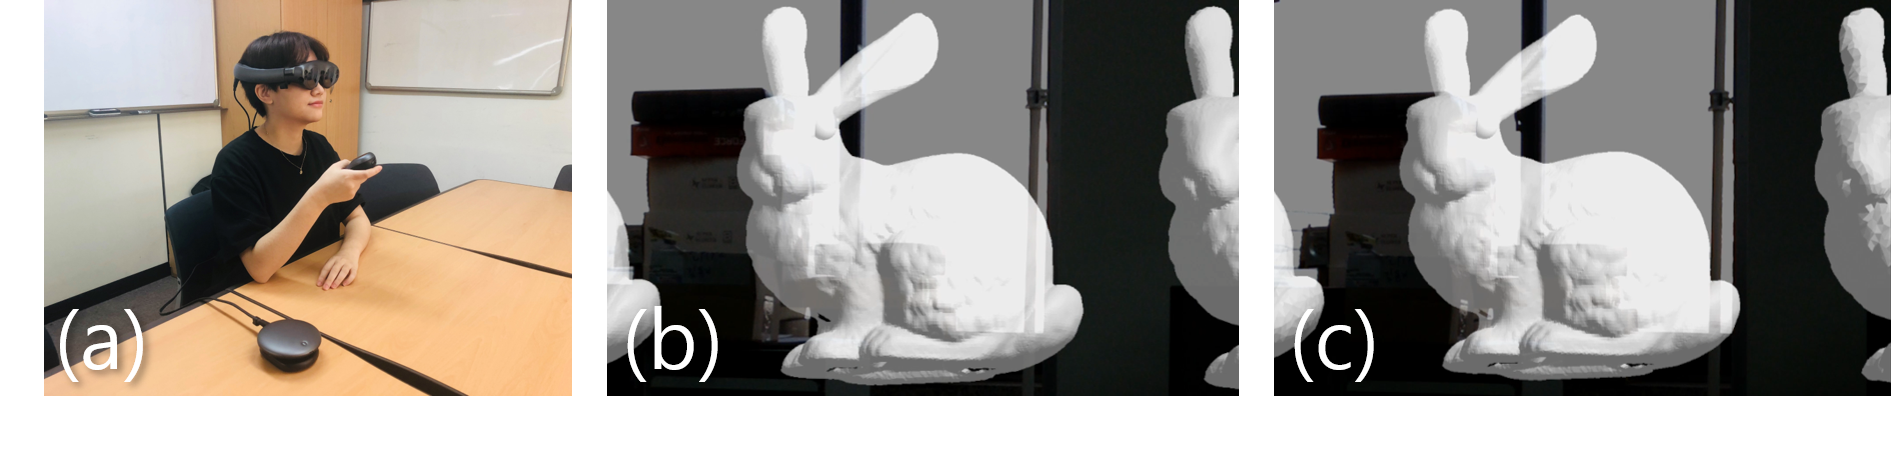
\includegraphics[width=1\linewidth]{comparison}
    \vspace{-4ex}
    \caption{Study participant with {\mlo} (a) with scenes observed from baseline (b) and {\myit} (c).}
    \label{fig:comparison}
\end{figure}



The primary goal of this work is to provide a solution that would work across 
various AR devices -- regardless of their manufacturer and software setup.
%
As such, we focused on adapting software and device aspects only those that
are accessible across all AR devices we surveyed. 
%(Section~\ref{sec:background})
%for survey results).
%
%From our survey, w
We found that most AR devices use proprietary software that
provides limited access to the hardware of the AR device. 
%
In particular, the head, eye, hand, and inertial tracking subsystems of these
AR devices were not easily modifiable -- you could read their values easily
but there was no access to change their settings to, for example, 
implement a duty cycling scheme.
%
However, all the surveyed devices provided OpenGL graphics libraries that
allowed good access to the rendering subsystems. Thus, to be as device 
independent as possible, we focused our efforts primarily on the rendering 
subsystems (while using inputs from the sensing components to drive our
adaptation) and defer adaptation of other energy-consuming components to 
future work -- or such a time where easy access to these subsystems becomes 
possible.

For this reason, {\myit} provides an OpenGL ES 3.0 compatible graphics API 
wrapper that is used to modify the application's OpenGL API calls to output 
a modified command set that reduces system-level power consumption.
%
This allows {\myit} to be highly device- and application- independent, 
and as transparent as possible to both applications and users.
%
Note: users may see a different output when {\myit} is enabled (especially if 
more aggressive power saving modes are selected) 
-- however this new output is still sufficient and acceptable for the task 
the user is performing and minimally disturbing within the user's core focal angle.
%
\fig\ref{fig:comparison} shows a sample scene presented using the baseline and {\myit}.


%%%%%%%%%%%%%%%%%%%%%%%%%%%%%%%%%%%%%%%%%%%%%%%%%%%%%%%%%%%%%%%%%%%%%%%%%%%%%%%%

We implemented {\myit} on the {\mlo}~\cite{magicleapone} (Section~\ref{sec:inlab})
and conducted an extensive set of in-lab experiments to evaluate its
system-level performance under various configurations.
%
In addition, we performed an IRB-approved user study with 25 student participants
to understand the usability impact of {\myit} (Section~\ref{sec:userstudies}).
%(c.f., \fig\ref{}).
%
%For this we conduct an Institutional Review Board (IRB) approved pilot %study
%with 25 university students.
%
Our results from in-lab experiments and the user study show that {\myit}
reduces the power usage by as much as $\sim$22\% 
with only marginal ($\sim$46$\mu$sec) added latency per displayed 
object on a frame and minimal loss in subjective user experience levels.
%
This power reduction translates to achieving 3.9 hours of continuous system lifetime, compared to 3.0 hours when using the baseline graphics library directly.
%
Furthermore, our experiments show that {\myit} results in similar or lower device 
temperature with the baseline approach while achieving higher frame rates.
%(Section~\ref{sec:eval}).

The major contributions of this paper are as follows:

\begin{itemize}[leftmargin=*]

    \item Detailed power measurements of {\mlo}, a commercial AR device, to inform and guide the design of {\myit}.

    \item Combining mobility features with rendering techniques to allow {\myit} to reduce GPU and memory usage power costs in a scalable manner.

    \item Detailed in-lab power and device temperature measurements showing the efficacy of {\myit}.

    \item Results from a 25 participant user study showing that {\myit} does not impact usability, accuracy, or task times.

\end{itemize}



%%%%%%%%%%%%%%%%%%%%%%%%%%%%%%%%%%%%%%%%%%%%%%%%%%%%%%%%%%%%%%%%%%%%%%%%%%%%%%%%

% Specifically, this paper makes the following contributions.
% %
% \vspace{-0.5ex}
% \begin{itemize}[leftmargin=*]
% %
%     \item We perform in-depth analysis on energy consumption patterns of 
%         an untethered AR HMD platform. We show that object complexity, frame rate and 
%         the number of draw calls heavily affect AR HMD's energy usage.
%         (Sec.~\ref{sec:preliminary})
    
%     \item We present {\myit}, an OpenGL API compatible library for
%         enhancing AR HMD's energy efficiency.
%         It uses the gyroscope to infer user perception, and transparently
%         modifies graphics operations to be more energy efficient.
%         (Sec.~\ref{sec:system}).
    
%     \item We conduct a comprehensive set of in-lab experiments as well as pilot 
%         deployments at an ophthalmology department in a university hospital.
%         Results show that 
%         {\myit} effectively reduces the AR HMD's energy usage while
%         minimally affecting latency and user experience. 
%         (Sec.~\ref{sec:app} and~\ref{sec:eval})
        
% \end{itemize}

%%%%%%%%%%%%%%%%%%%%%%%%%%%%%%%%%%%%%%%%%%%%%%%%%%%%%%%%%%%%%%%%%%%%%%%%%%%%%%%%

% The remainder of this paper is structured as follows.
% %
% We first present a preliminary study on the energy usage of AR HMD platform in
% Section~\ref{sec:preliminary}, which motivates and guides our design of {\myit}.
% %
% We then describe the design and key ideas of {\myit} in Section~\ref{sec:system},
% and discuss the implementation issues in Section~\ref{sec:implementation}.
% %
% We evaluate our system in Section~\ref{sec:eval}, 
% discuss related work in Section~\ref{sec:related},
% and conclude the work in Section~\ref{sec:conclusion}.

%%%%%%%%%%%%%%%%%%%%%%%%%%%%%%%%%%%%%%%%%%%%%%%%%%%%%%%%%%%%%%%%%%%%%%%%%%%%%%%%

